\chapter{Introduction}\label{introduction}
Bla Bla

\begin{figure}[!htb]
\begin{center}
	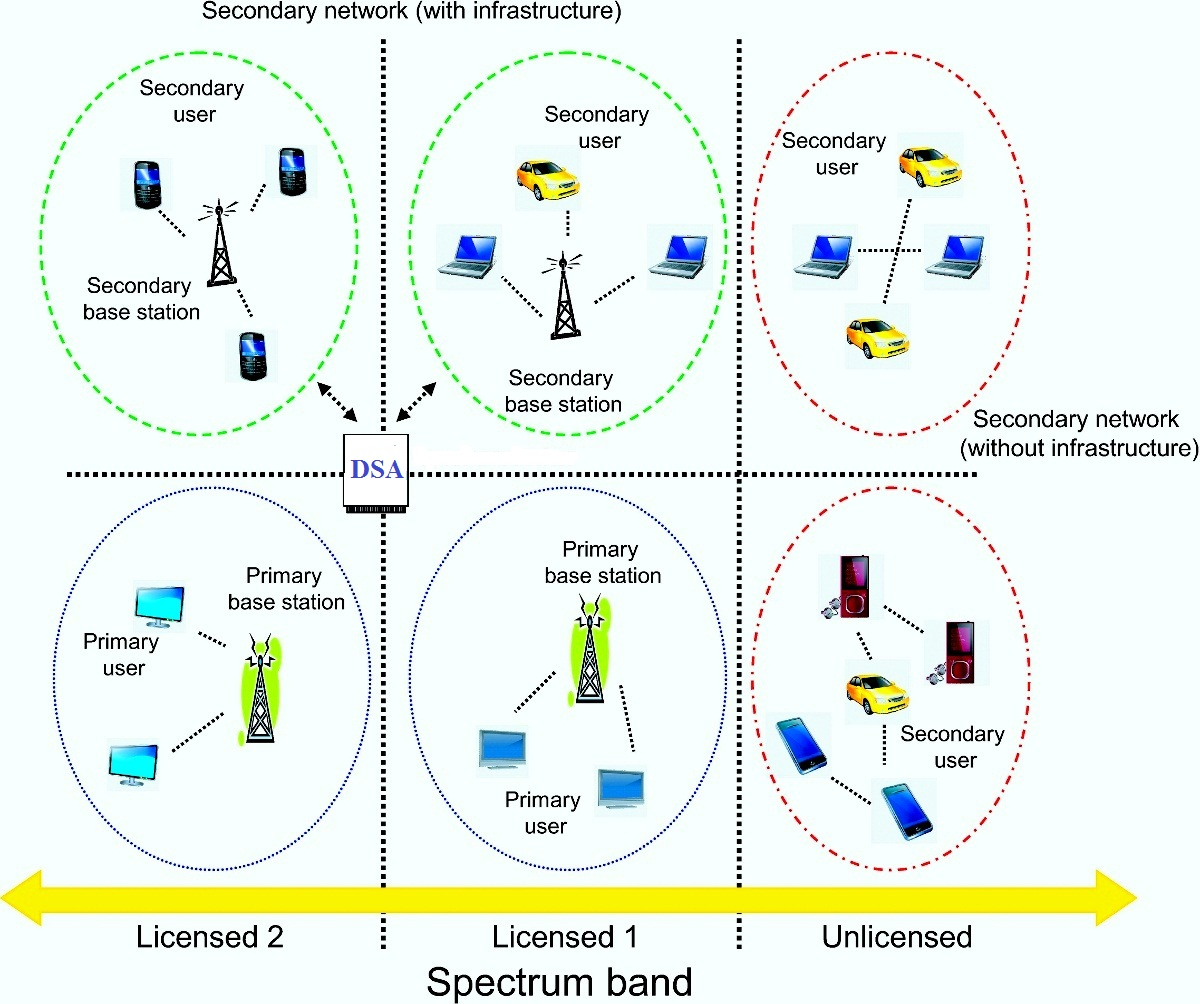
\includegraphics[scale=0.5]{figures/crn.jpg}
	\caption{Cognitive Radio Network (CRN) architecture (source: \cite{r17})}
	\label{fig:crn}
\end{center}
%\vspace{-5mm}
\end{figure}



  
\begin{figure}[!htb]
\vspace{3mm}
\begin{center}
	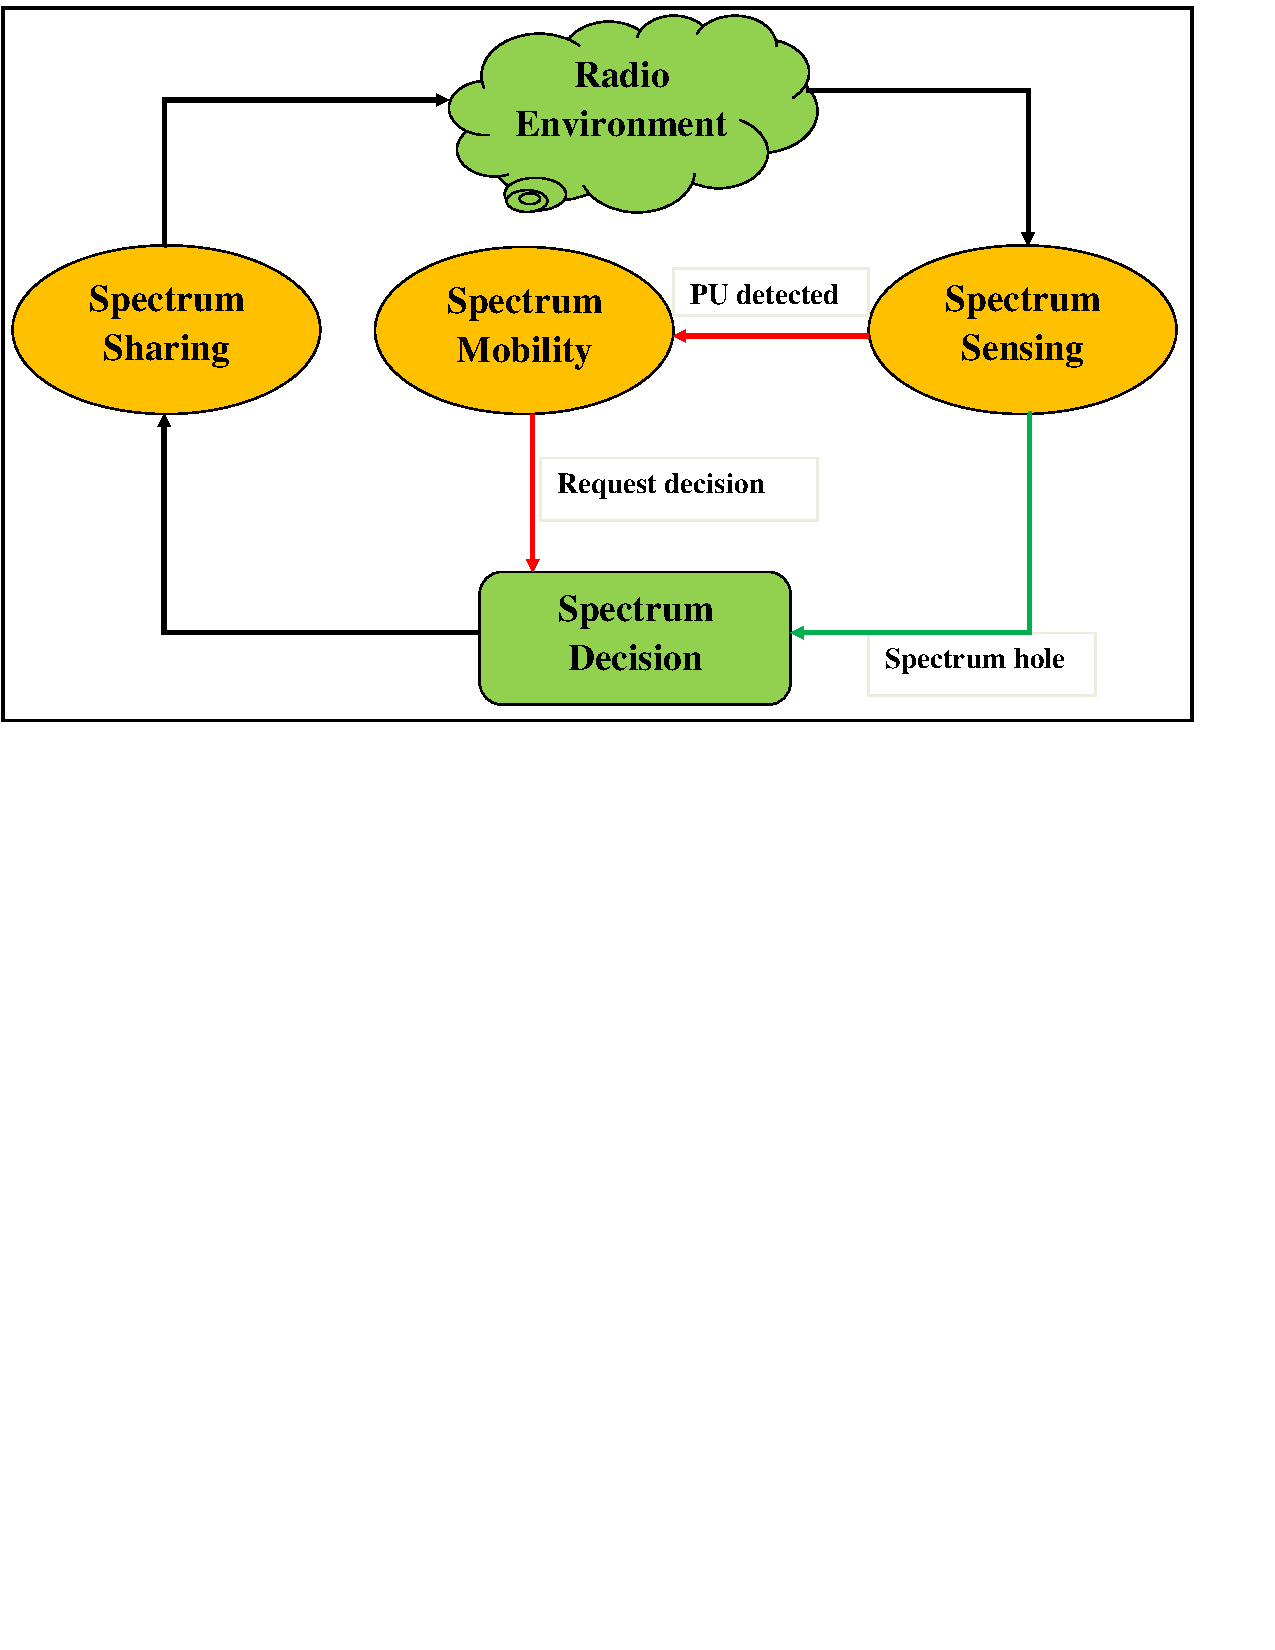
\includegraphics[scale=0.5]{figures/DSA.pdf}
	\vspace{-78mm}
	\caption{Mechanism of DSA}
	\label{fig:DSA}
\end{center}
\vspace{-7mm}
\end{figure}

In this thesis, we design a novel hybrid DSA technique for multi-channel single-radio CRNs. Designing efficient DSA techniques for CRNs has been a well-researched topic in recent years. In the following sections, we discuss the motivations and contributions of our work in this affair.



\section{Motivations of Our Work}
Bla Bla

\begin{table}[!thb]
\vspace{2mm}
\begin{center}
%\begin{minipage}{0.5\textwidth}
\caption{Pros and cons of the state-of-art DSA techniques in CRNs}\vspace{-2mm}
\begin{tabular}{|c|c|c|}
\hline
\textbf{Issues} & \textbf{Classical approaches} & \textbf{Stochastic approaches} \\
\hline \hline
Scalability & Limited & Ok \\
 \hline
Ease of Formulation & Limited & Ok \\
 \hline
 Robustness & Limited & Ok \\
 \hline
Consideration of PUs & Not always & Ok \\
 \hline
 Convergence & Ok & Not always \\
 \hline
 Problem Specific Operator/Parameter Design & Ok & Not always \\
\hline
\end{tabular}
%\vspace{-3mm}
\label{iss}
%\end{minipage}
\end{center}
\end{table}


\section{Our Contributions}
Bla Bla

\section{Outline of Our Thesis}
This is how the rest of this book is organized. In Chapter~\ref{sec:previousworks}, we elaborate on the background of the DSA problem in CRNs  and analyse this problem from different viewpoints highlighting related works in each cases. Then, in Chapter \ref{sec:NetM}, we present the network model and summarise the modifications that we performed in the basic CRCN simulator. Next to that, we investigate the performance of GA-based DSA with basic genetic operators in Chapter \ref{sec:Pf}. On the basis of results found from this chapter, we devise novel genetic operators that we use in GALS. We present these novel genetic operators in Chapter \ref{sec:Nf}. Then, we illustrate the detailed GALS algorithm and compute its computational complexity in Chapter \ref{sec:algo}. Finally, in Chapter \ref{sec:Er}, we present a comprehensive analysis of the performance of GALS algorithm in terms various QoS parameters. This chapter also include the performance comparison of GALS with other state-of-the-art algorithms and findings of our simulation results. At last, we draw our conclusions and present possible future studies in Chapter~\ref{conclusion}.
